\section{Embedded Linux system development}

\begin{frame}
  \frametitle{Contents}
  \begin{itemize}
  \item Using open-source components
  \item Tools for the target device
    \begin{itemize}
    \item Networking
    \item System utilities
    \item Language interpreters
    \item Audio, video and multimedia
    \item Graphical toolkits
    \item Databases
    \item Web browsers
    \end{itemize}
  \item System building
  \end{itemize}
\end{frame}

\subsection{Leveraging open-source components in an Embedded Linux
  system}

\begin{frame}
  \frametitle{Third party libraries and applications}
  \begin{itemize}
  \item One of the advantages of embedded Linux is the wide range of
    third-party libraries and applications that one can leverage in
    its product
    \begin{itemize}
    \item They are freely available, freely distributable, and thanks
      to their open-source nature, they can be analyzed and modified
      according to the needs of the project
    \end{itemize}
  \item However, efficiently re-using these components is not always
    easy. One must:
    \begin{itemize}
    \item Find these components
    \item Choose the most appropriate ones
    \item Cross-compile them
    \item Integrate them in the embedded system and with the other
      applications
    \end{itemize}
  \end{itemize}
\end{frame}

\begin{frame}
  \frametitle{Find existing components}
  \begin{itemize}
  \item Free Software Directory\\
    \url{http://directory.fsf.org}
  \item Look at other embedded Linux products, and see what their
    components are
  \item Look at the list of software packaged by embedded Linux build
    systems
    \begin{itemize}
    \item These are typically chosen for their suitability to embedded
      systems
    \end{itemize}
  \item Ask the community or Google
  \item This presentation will also feature a list of components for
    common needs
  \end{itemize}
\end{frame}

\begin{frame}
  \frametitle{Choosing components}
  Not all free software components are necessarily good to
  re-use. One must pay attention to:
  \begin{itemize}
  \item {\bf Vitality} of the developer and user communities. This
    vitality ensures long-term maintenance of the component, and
    relatively good support. It can be measured by looking at the
    mailing-list traffic and the version control system activity.
  \item {\bf Quality} of the component. Typically, if a component is
    already available through embedded build systems, and has a
    dynamic user community, it probably means that the quality is
    relatively good.
  \item {\bf License}. The license of the component must match your
    licensing constraints. For example, GPL libraries cannot be used
    in proprietary applications.
  \item {\bf Technical requirements}. Of course, the component must
    match your technical requirements. But don't forget that you can
    improve the existing components if a feature is missing!
  \end{itemize}
\end{frame}

\begin{frame}
  \frametitle{Licenses (1)}
  \begin{itemize}
  \item All software that are under a free software license give four
    freedoms to all users
    \begin{itemize}
    \item Freedom to use
    \item Freedom to study
    \item Freedom to copy
    \item Freedom to modify and distribute modified copies
    \end{itemize}
  \item See \url{http://www.gnu.org/philosophy/free-sw.html} for a
    definition of Free Software
  \item Open Source software, as per the definition of the Open Source
    Initiative, are technically similar to Free Software in terms of
    freedoms
  \item See \url{http://www.opensource.org/docs/osd} for the definition of
    Open Source Software
  \end{itemize}
\end{frame}

\begin{frame}
  \frametitle{Licenses (2)}
  \begin{columns}
    \column{0.8\textwidth}
    \begin{itemize}
      \item Free Software licenses fall in two main categories
      \begin{itemize}
      \item The copyleft licenses
      \item The non-copyleft licenses
      \end{itemize}
    \item The concept of {\em copyleft} is to ask for reciprocity in the
      freedoms given to a user.
    \item The result is that when you receive a software under a
      copyleft free software license and distribute modified versions of
      it, you must do so under the same license
      \begin{itemize}
      \item Same freedoms to the new users
      \item It's an incentive to contribute back your changes instead of
        keeping them secret
      \end{itemize}
    \item Non-copyleft licenses have no such requirements, and modified
      versions can be kept proprietary, but they still require
      attribution
    \end{itemize}
    \column{0.2\textwidth}
    
\includegraphics[width=\textwidth]{slides/sysdev-embedded-linux/copyleft.pdf}
  \end{columns} 
\end{frame}

\begin{frame}
  \frametitle{GPL}
  \begin{itemize}
  \item {\bf GNU General Public License}
    \hfill 
\includegraphics[width=6em]{slides/sysdev-embedded-linux/gpl-v3.pdf}
  \item Covers around 55\% of the free software projects
    \begin{itemize}
    \item Including the Linux kernel, Busybox and many applications
    \end{itemize}
  \item Is a copyleft license
    \begin{itemize}
    \item Requires derivative works to be released under the same
      license
    \item Programs linked with a library released under the GPL must
      also be released under the GPL
    \end{itemize}
  \item Some programs covered by version 2 (Linux kernel, Busybox and
    others)
  \item More and more programs covered by version 3, released in 2007
    \begin{itemize}
    \item Major change for the embedded market: the requirement that
      the user must be able to {\bf run} the modified versions on the
      device, if the device is a {\em consumer} device
    \end{itemize}
  \end{itemize}
\end{frame}

\begin{frame}
  \frametitle{GPL: redistribution}
  \begin{itemize}
  \item No obligation when the software is not distributed
    \begin{itemize}
    \item You can keep your modifications secret until the product
      delivery
    \end{itemize}
  \item It is then authorized to distribute binary versions, if one of
    the following conditions is met:
    \begin{itemize}
    \item Convey the binary with a copy of the source on a physical
      medium
    \item Convey the binary with a written offer valid for 3 years
      that indicates how to fetch the source code
    \item Convey the binary with the network address of a location
      where the source code can be found
    \item See section 6. of the GPL license
    \end{itemize}
  \item In all cases, the attribution and the license must be
    preserved
    \begin{itemize}
    \item See section 4. and 5.
    \end{itemize}
  \end{itemize}
\end{frame}

\begin{frame}
  \frametitle{LGPL}
  \begin{itemize}
  \item {\bf GNU Lesser General Public License}
    \hfill 
\includegraphics[width=6em]{slides/sysdev-embedded-linux/lgpl-v3.pdf}
  \item Covers around 10\% of the free software projects
  \item A copyleft license
    \begin{itemize}
    \item Modified versions must be released under the same license
    \item But, programs linked against a library under the LGPL do not
      need to be released under the LGPL and can be kept proprietary.
    \item However, the user must keep the ability to update the
      library independently from the program. Dynamic linking is the
      easiest solution. Statically linked executables are only possible
      if the developer provides a way to relink with an update
      (with source code or linkable object files).
    \end{itemize}
  \item Used instead of the GPL for most of the libraries, including
    the C libraries
    \begin{itemize}
    \item Some exceptions: MySQL, or Qt \textless = 4.4
    \end{itemize}
  \item Also available in two versions, v2 and v3
  \end{itemize}
\end{frame}

\begin{frame}
  \frametitle{Licensing: examples}
  \begin{itemize}
  \item You make modifications to the Linux kernel (to add drivers or
    adapt to your board), to Busybox, U-Boot or other GPL software
    \begin{itemize}
    \item You must release the modified versions under the same
      license, and be ready to distribute the source code to your
      customers
    \end{itemize}
  \item You make modifications to the C library or any other LGPL
    library
    \begin{itemize}
    \item You must release the modified versions under the same
      license
    \end{itemize}
  \item You create an application that relies on LGPL libraries
    \begin{itemize}
    \item You can keep your application proprietary, but you must link
      dynamically with the LGPL libraries
    \end{itemize}
  \item You make modifications to a non-copyleft licensed software
    \begin{itemize}
    \item You can keep your modifications proprietary, but you must
      still credit the authors
    \end{itemize}
  \end{itemize}
\end{frame}

\begin{frame}
  \frametitle{Non-copyleft licenses}
  \begin{itemize}
  \item A large family of non-copyleft licenses that are relatively
    similar in their requirements
  \item A few examples
    \begin{itemize}
    \item Apache license (around 4\%)
    \item BSD license (around 6\%)
    \item MIT license (around 4\%)
    \item X11 license
    \item Artistic license (around 9 \%)
    \end{itemize}
  \end{itemize}
\end{frame}

\begin{frame}[fragile]
  \frametitle{BSD license}
  \begin{block}{}
  \tiny
  \begin{verbatim}
Copyright (c) <year>, <copyright holder>
All rights reserved.

Redistribution and use in source and binary forms, with or without
modification, are permitted provided that the following conditions are
met:
* Redistributions of source code must retain the above copyright
  notice, this list of conditions and the following disclaimer.
* Redistributions in binary form must reproduce the above copyright
  notice, this list of conditions and the following disclaimer in the
  documentation and/or other materials provided with the distribution.
* Neither the name of the <organization> nor the names of its
  contributors may be used to endorse or promote products derived from
  this software without specific prior written permission.

[...]
\end{verbatim}
  \end{block}
\end{frame}

\begin{frame}
  \frametitle{Is this free software?}
  \begin{itemize}
  \item Most of the free software projects are covered by ~10
    well-known licenses, so it is fairly easy for the majority of
    projects to get a good understanding of the license
  \item Otherwise, read the license text
  \item Check Free Software Foundation's opinion\\
    \url{http://www.fsf.org/licensing/licenses/}
  \item Check Open Source Initiative's opinion\\
    \url{http://www.opensource.org/licenses}
  \end{itemize}
\end{frame}

\begin{frame}
  \frametitle{Respect free software licenses}
  \begin{itemize}
  \item Free Software is not public domain software, the distributors
    have obligations due to the licenses
    \begin{itemize}
    \item {\bf Before} using a free software component, make sure the
      license matches your project constraints
    \item Make sure to keep a complete list of the free software
      packages you use, the original version numbers you used, and to
      keep your modifications and adaptations well-separated from
      the original version.
    \item Buildroot and Yocto Project can generate this list for you!
    \item Conform to the license requirements before shipping the
      product to the customers.
    \end{itemize}
  \item Free Software licenses have been enforced successfully in
    courts. Organizations which can help:
    \begin{itemize}
    \item Software Freedom Law Center, \url{http://www.softwarefreedom.org/}
    \item Software Freedom Conservancy, \url{http://sfconservancy.org/}
    \end{itemize}
  \item Ask your legal department!
  \end{itemize}
\end{frame}

\begin{frame}
  \frametitle{Keeping changes separate (1)}
  \begin{itemize}
  \item When integrating existing open-source components in your
    project, it is sometimes needed to make modifications to them
    \begin{itemize}
    \item Better integration, reduced footprint, bug fixes, new
      features, etc.
    \end{itemize}
  \item Instead of mixing these changes, it is much better to keep
    them separate from the original component version
    \begin{itemize}
    \item If the component needs to be upgraded, easier to know what
      modifications were made to the component
    \item If support from the community is requested, important to
      know how different the component we're using is from the
      upstream version
    \item Makes contributing the changes back to the community
      possible
    \end{itemize}
  \item It is even better to keep the various changes made on a given
    component separate
    \begin{itemize}
    \item Easier to review and to update to newer versions
    \end{itemize}
  \end{itemize}
\end{frame}

\begin{frame}
  \frametitle{Keeping changes separate (2)}
  \begin{itemize}
  \item The simplest solution is to use Quilt
    \begin{itemize}
    \item Quilt is a tool that allows to maintain a stack of patches
      over source code
    \item Makes it easy to add, remove modifications from a patch, to
      add and remove patches from stack and to update them
    \item The stack of patches can be integrated into your version
      control system
    \item \url{https://savannah.nongnu.org/projects/quilt/}
    \end{itemize}
  \item Another solution is to use a version control system
    \begin{itemize}
    \item Import the original component version into your version
      control system
    \item Maintain your changes in a separate branch
    \end{itemize}
  \end{itemize}
\end{frame}

\subsection[Networking tools]{Tools for the target device: Networking}

\begin{frame}
  \frametitle{ssh server and client: Dropbear}
  \url{http://matt.ucc.asn.au/dropbear/dropbear.html}
  \begin{itemize}
  \item Very small memory footprint ssh server for embedded systems
  \item Satisfies most needs. Both client and server!
  \item Size: 110 KB, statically compiled with uClibc on x86.\\
    (OpenSSH client and server: approx 1200 KB, dynamically compiled
    with glibc on x86)
  \item Useful to:
    \begin{itemize}
    \item Get a remote console on the target device
    \item Copy files to and from the target device (\code{scp} or
      \code{rsync -e ssh}).
    \end{itemize}
  \item An alternative to OpenSSH, used on desktop and server systems.
  \end{itemize}
\end{frame}

\begin{frame}
  \frametitle{Benefits of a web server interface}

  Many network enabled devices can just have a network interface

  \begin{itemize}
  \item Examples: modems / routers, IP cameras, printers...
  \item No need to develop drivers and applications for computers
    connected to the device. No need to support multiple operating
    systems!
  \item Just need to develop static or dynamic HTML pages (possibly
    with powerful client-side JavaScript).\\
    Easy way of providing access to device information and parameters.
  \item Reduced hardware costs (no LCD, very little storage space
    needed)
  \end{itemize}
\end{frame}

\begin{frame}
  \frametitle{Web servers}
  \begin{columns}
    \column{0.8\textwidth}
    \begin{itemize}
    \item {\em BusyBox http server}: \url{http://busybox.net}
      \begin{itemize}
      \item Tiny: only adds 9 K to BusyBox (dynamically linked with
        glibc on x86, with all features enabled.)
      \item Sufficient features for many devices with a web interface,
        including CGI, http authentication and script support (like
        PHP, with a separate interpreter).
      \item License: GPL
      \end{itemize}
    \item Other possibilities: lightweight servers like {\em Boa},
          {\em thttpd}, {\em lighttpd}, {\em nginx}, etc
    \item Some products are using {\em Node.js}, which is lightweight
          enough to be used.
    \end{itemize}
    \column{0.2\textwidth}
    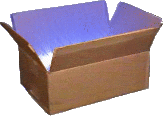
\includegraphics[width=0.9\textwidth]{slides/sysdev-embedded-linux/busybox.png}\\
  \end{columns}
\end{frame}

\begin{frame}
  \frametitle{Network utilities (1)}
  \begin{itemize}
  \item {\bf avahi} is an implementation of Multicast DNS Service
    Discovery, that allows programs to publish and discover services
    on a local network
  \item {\bf bind}, a DNS server
  \item {\bf iptables}, the user space tools associated to the Linux firewall, Netfilter
  \item {\bf iw and wireless tools}, the user space tools associated to Wireless devices
  \item {\bf netsnmp}, implementation of the SNMP protocol
  \item {\bf openntpd}, implementation of the Network Time Protocol,
    for clock synchronization
  \item {\bf openssl}, a toolkit for SSL and TLS connections
  \end{itemize}
\end{frame}

\begin{frame}
  \frametitle{Network utilities (2)}
  \begin{itemize}
  \item {\bf pppd}, implementation of the Point to Point Protocol,
    used for dial-up connections
  \item {\bf samba}, implements the SMB and CIFS protocols, used by
    Windows to share files and printers
  \item {\bf coherence}, a UPnP/DLNA implementation
  \item {\bf vsftpd}, proftpd, FTP servers
  \end{itemize}
\end{frame}

\subsection[System utilities]{Tools for the target device: System
  utilities}

\begin{frame}
  \frametitle{System utilities}
  \begin{itemize}
  \item {\bf dbus}, an inter-application object-oriented communication bus
  \item {\bf gpsd}, a daemon to interpret and share GPS data
  \item {\bf libraw1394}, raw access to Firewire devices
  \item {\bf libusb}, a user space library for accessing USB devices
    without writing an in-kernel driver
  \item Utilities for kernel subsystems: {\bf i2c-tools} for I2C, {\bf
      input-tools} for input, {\bf mtd-utils} for MTD devices, {\bf
      usbutils} for USB devices
  \end{itemize}
\end{frame}

\subsection[Language Interpreters]{Tools for the target device:
  Language interpreters}

\begin{frame}
  \frametitle{Language interpreters}
  \begin{itemize}
  \item Interpreters for the most common scripting languages are
    available. Useful for
    \begin{itemize}
    \item Application development
    \item Web services development
    \item Scripting
    \end{itemize}
  \item Languages supported
    \begin{itemize}
    \item Lua
    \item Python
    \item Perl
    \item Ruby
    \item TCL
    \item PHP
    \end{itemize}
  \end{itemize}
\end{frame}

\subsection[Multimedia tools]{Tools for the target device: Audio,
  video and multimedia}

\begin{frame}
  \frametitle{Audio, video and multimedia}
  \begin{itemize}
  \item {\bf GStreamer}, a multimedia framework
    \begin{itemize}
    \item Allows to decode/encode a wide variety of codecs.
    \item Supports hardware encoders and decoders through plugins,
      proprietary/specific plugins are often provided by SoC vendors.
    \end{itemize}
  \item {\bf alsa-lib}, the user space tools associated to the ALSA sound
    kernel subsystem
  \item Directly using encoding and decoding libraries, if you decide
    not to use GStreamer: libavcodec, libogg, libtheora, libvpx, flac
    (lossless audio compression), libvorbis, libopus (better than vorbis!),
    libmad, libsndfile, speex (for human speech), etc.
  \end{itemize}
\end{frame}

\subsection[Graphical toolkits]{Tools for the target device: Graphical
  toolkits}

\subsection[Low-level toolkits]{Graphical toolkits:
``Low-level'' solutions and layers}

\begin{frame}
  \frametitle{X.org - KDrive}
  \begin{columns}[T]
    \column{0.8\textwidth}
    \begin{itemize}
    \item Stand-alone simplified version of the X server, for embedded
      systems
      \begin{itemize}
      \item Formerly know as Tiny-X
      \item Kdrive is integrated in the official X.org server
      \end{itemize}
    \item Works on top of the Linux frame buffer, thanks to the Xfbdev
      variant of the server
    \item Real X server
      \begin{itemize}
      \item Fully supports the X11 protocol: drawing, input event
        handling, etc.
      \item Allows to use any existing X11 application or library
      \end{itemize}
    \item Actively developed and maintained.
    \item X11 license
    \item \url{http://www.x.org}
    \end{itemize}
    \column{0.2\textwidth}
    
\includegraphics[width=\textwidth]{slides/sysdev-embedded-linux/xorg.pdf}
  \end{columns}
\end{frame}

\begin{frame}
  \frametitle{Kdrive: architecture}
  \begin{center}
    \includegraphics[height=0.8\textheight]{slides/sysdev-embedded-linux/xorg-architecture.pdf}
  \end{center}
\end{frame}

\begin{frame}
  \frametitle{Kdrive: usage}
  \begin{itemize}
  \item Can be directly programmed using Xlib / XCB
    \begin{itemize}
    \item Low-level graphic library, rarely used
    \end{itemize}
  \item Or, usually used with a toolkit on top of it
    \begin{itemize}
    \item Gtk
    \item Qt
    \item Enlightenment Foundation Libraries
    \item Others: Fltk, WxEmbedded, etc
    \end{itemize}
  \end{itemize}
\end{frame}

\begin{frame}
  \frametitle{Wayland}
  \begin{columns}[T]
    \column{0.8\textwidth}
    \begin{itemize}
    \item Intended to be a simpler replacement for X
    \item {\em Wayland is a protocol for a compositor to talk to
    its clients as well as a C library implementation of that protocol.}
    \item Weston: a minimal and fast reference implementation
          of a Wayland compositor, and is suitable for many embedded
          and mobile use cases.
    \item Not fully deployed yet. However, the ports of Gtk and Qt
          to Wayland are complete.
    \item \url{http://wayland.freedesktop.org/}
    \end{itemize}
    \column{0.2\textwidth}
    
\includegraphics[width=\textwidth]{slides/sysdev-embedded-linux/wayland.png}
  \end{columns}
\end{frame}

\begin{frame}
  \frametitle{Wayland: architecture}
  \begin{center}
    \includegraphics[height=0.8\textheight]{slides/sysdev-embedded-linux/wayland-architecture.pdf}
  \end{center}
\end{frame}


\subsection[High-level Toolkits]{Graphical toolkits: ``High-level''
  solutions}

\begin{frame}
  \frametitle{Gtk}
  \begin{columns}
    \column{0.8\textwidth}
    \begin{itemize}
    \item The famous toolkit, providing widget-based high-level APIs to
      develop graphical applications
    \item Standard API in C, but bindings exist for various languages:
      C++, Python, etc.
    \item Works on top of X.org and Wayland.
    \item No windowing system, a lightweight window manager needed to
      run several applications. Possible solution: Matchbox.
    \item License: LGPL
    \item Multiplatform: Linux, MacOS, Windows.
    \item \url{http://www.gtk.org}
    \end{itemize}
    \column{0.2\textwidth}
    \includegraphics[width=0.8\textwidth]{slides/sysdev-embedded-linux/gtk-backends.pdf}
  \end{columns}
\end{frame}

\begin{frame}
  \frametitle{Gtk stack components}
  \begin{itemize}
  \item {\bf Glib}, core infrastructure
    \begin{itemize}
    \item Object-oriented infrastructure GObject
    \item Event loop, threads, asynchronous queues, plug-ins, memory
      allocation, I/O channels, string utilities, timers, date and
      time, internationalization, simple XML parser, regular
      expressions
    \item Data types: memory slices and chunks, linked lists, arrays,
      trees, hash tables, etc.
    \end{itemize}
  \item {\bf Pango}, internationalization of text handling
  \item {\bf ATK}, accessibility toolkit
  \item {\bf Cairo}, vector graphics library
  \item {\bf Gtk+}, the widget library itself
  \item {\em The Gtk stack is a complete framework to develop applications}
  \end{itemize}
\end{frame}

\begin{frame}
  \frametitle{Gtk example}
    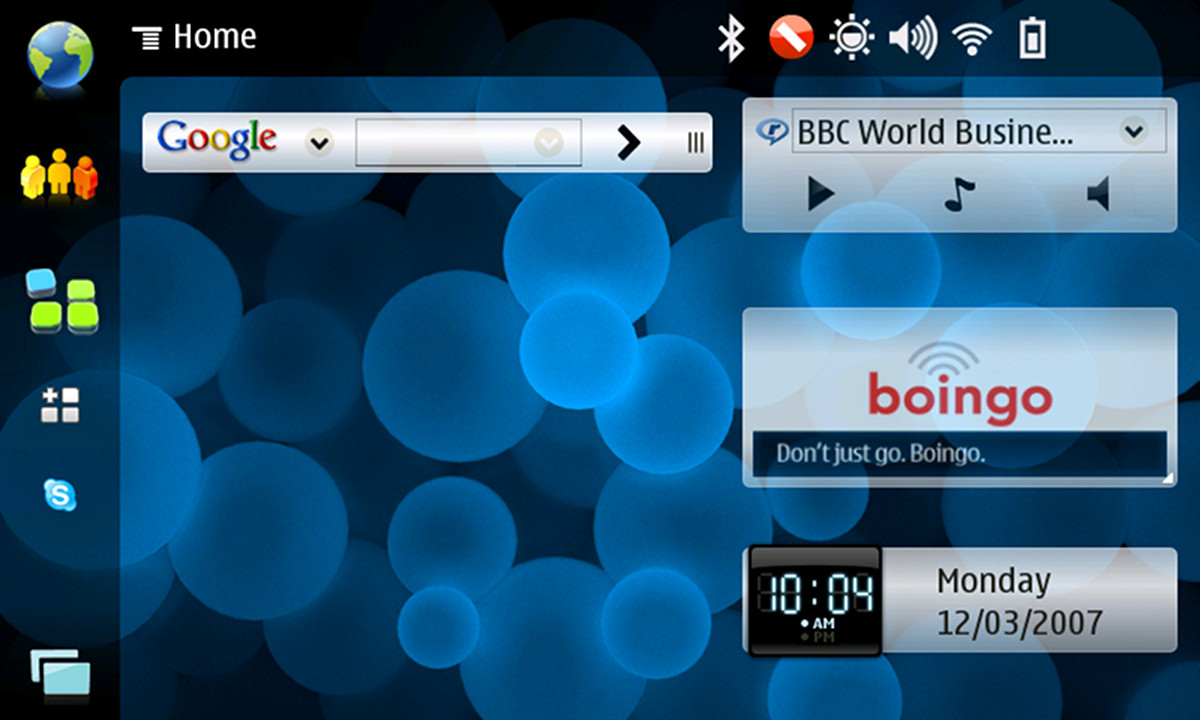
\includegraphics[height=0.6\textheight]{slides/sysdev-embedded-linux/maemo-gui.jpg}\\
    Maemo tablet / phone interface\\
    GTK is losing traction, however:
    Mer, the descendent of Maemo, is now implemented in EFL (see next
    slides).\\
\end{frame}

\begin{frame}
  \frametitle{Qt (1)}
  \begin{itemize}
  \item The other famous toolkit, providing widget-based high-level APIs to
    develop graphical applications
  \item Implemented in C++
    \begin{itemize}
    \item the C++ library is required on the target system
    \item standard API in C++, but with bindings for other languages
    \end{itemize}
  \item Works either on top of
    \begin{itemize}
    \item Framebuffer
    \item X11
    \item Wayland
    \end{itemize}
  \item Multiplatform: Linux, MacOS, Windows.
  \end{itemize}
\end{frame}

\begin{frame}
  \frametitle{Qt (2)}
  \begin{itemize}
  \item Qt is more than just a graphical toolkit, it also offers a
    complete development framework: data structures, threads, network,
    databases, XML, etc.
  \item See our presentation {\em Qt for non graphical applications}
    presentation at ELCE 2011 (Thomas Petazzoni):
    \url{http://j.mp/W4PK85}
  \item Qt Embedded has an integrated windowing system, allowing
    several applications to share the same screen
  \item Very well documented
  \item Since version 4.5, available under the LGPL, allowing
    proprietary applications
  \item Since version 4.7, LGPL v2 is dropped, leaving LGPLv3 and
        GPLv3 (and GPLv2 for some parts) as only options, which add
        more restrictions to proprietary applications.
  \end{itemize}
\end{frame}

\begin{frame}
  \frametitle{Qt's usage}
  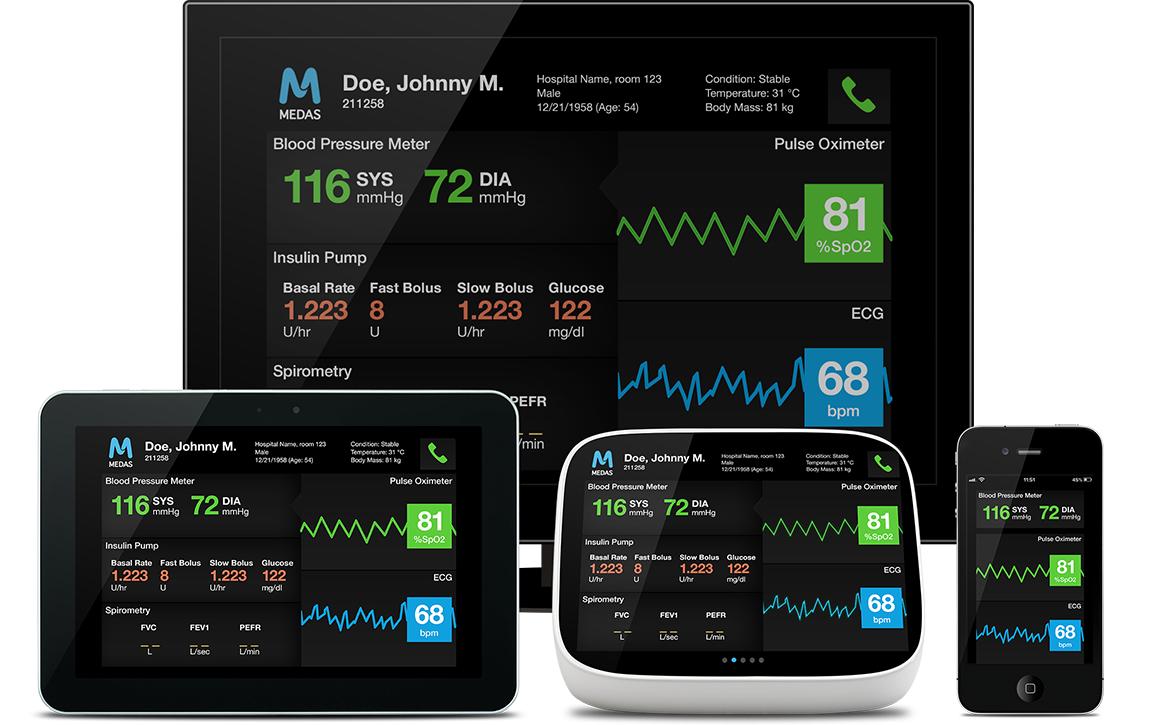
\includegraphics[width=\textwidth]{slides/sysdev-embedded-linux/qt-devices.png}
  \vfill
  Source: \url{https://www.qt.io/qt-for-device-creation/}
\end{frame}

\begin{frame}
  \frametitle{Other less frequent solutions}
  \begin{itemize}
  \item Enlightenment Foundation Libraries (EFL)
    \begin{itemize}
    \item Very powerful. Supported by Samsung, Intel and Free.fr.
    \item Work on top of X or Wayland.
    \item \url{http://www.enlightenment.org/p.php?p=about/efl}
    \end{itemize}
  \end{itemize}
\end{frame}

\subsection[Databases]{Tools for the target device: Databases}

\begin{frame}
  \frametitle{Lightweight database - SQLite}
  \url{http://www.sqlite.org}

  \begin{itemize}
  \item SQLite is a small C library that implements a self-contained,
    embeddable, lightweight, zero-configuration SQL database engine
  \item The database engine of choice for embedded Linux systems
    \begin{itemize}
    \item Can be used as a normal library
    \item Can be directly embedded into a application, even a
      proprietary one since SQLite is released in the public domain
    \end{itemize}
  \end{itemize}
\end{frame}

\subsection[Web Browsers]{Tools for the target device: Web browsers}

\begin{frame}
  \frametitle{WebKit}
  \begin{columns}[T]
    \column{0.8\textwidth}
    \url{http://webkit.org/}
    \begin{itemize}
    \item Web browser engine. Application framework that can be used
      to develop web browsers.
    \item License: portions in LGPL and others in BSD. Proprietary
      applications allowed.
    \item Used by many web browsers: Safari, iPhone and Android default
      browsers ... Google Chrome now uses a fork of its WebCore component).
      Used by e-mail clients too to render HTML:
      \url{http://trac.webkit.org/wiki/Applications\%20using\%20WebKit}
    \item Multiple graphical back-ends: Qt4, GTK, EFL...
    \item You could use it to create your custom browser.
    \end{itemize}
    \column{0.2\textwidth}
    
\includegraphics[width=\textwidth]{slides/sysdev-embedded-linux/webkit.png}
  \end{columns}
\end{frame}

\subsection{System building}

\begin{frame}
  \frametitle{System building: goal and solutions}
  \begin{columns}
    \column{0.6\textwidth}
    \begin{itemize}
    \item Goal
      \begin{itemize}
      \item Integrate all the software components, both third-party and
        in-house, into a working root filesystem
      \item It involves the download, extraction, configuration,
        compilation and installation of all components, and possibly
        fixing issues and adapting configuration files
      \end{itemize}
    \item Several solutions
      \begin{itemize}
      \item Manually
      \item System building tools
      \item Distributions or ready-made filesystems
      \end{itemize}
    \end{itemize}
    \column{0.4\textwidth}
    
\includegraphics[width=\textwidth]{slides/sysdev-embedded-linux/lego-penguin.png}
    \vfill
    {\tiny Penguin picture: \url{http://bit.ly/1PwDklz}}
  \end{columns}
\end{frame}

\begin{frame}
  \frametitle{System building: manually}
  \begin{itemize}
  \item Manually building a target system involves downloading,
    configuring, compiling and installing all the components of the
    system.
  \item All the libraries and dependencies must be configured,
    compiled and installed in the right order.
  \item Sometimes, the build system used by libraries or applications
    is not very cross-compile friendly, so some adaptations are
    necessary.
  \item There is no infrastructure to reproduce the build from
    scratch, which might cause problems if one component needs to be
    changed, if somebody else takes over the project, etc.
  \end{itemize}
\end{frame}

\begin{frame}
  \frametitle{System building: manually (2)}
  \begin{itemize}
  \item Manual system building is not recommended for production
    projects
  \item However, using automated tools often requires the developer to
    dig into specific issues
  \item Having a basic understanding of how a system can be built
    manually is therefore very useful to fix issues encountered with
    automated tools
    \begin{itemize}
    \item We will first study manual system building, and during a
      practical lab, create a system using this method
    \item Then, we will study the automated tools available, and use
      one of them during a lab
    \end{itemize}
  \end{itemize}
\end{frame}

\begin{frame}
  \frametitle{System foundations}
  \begin{itemize}
  \item A basic root file system needs at least
    \begin{itemize}
    \item A traditional directory hierarchy, with \code{/bin},
      \code{/etc}, \code{/lib}, \code{/root}, \code{/usr/bin},
      \code{/usr/lib}, \code{/usr/share}, \code{/usr/sbin},
      \code{/var}, \code{/sbin}
    \item A set of basic utilities, providing at least the \code{init}
      program, a shell and other traditional Unix command line
      tools. This is usually provided by {\em Busybox}
    \item The C library and the related libraries (thread, math, etc.)
      installed in \code{/lib}
    \item A few configuration files, such as \code{/etc/inittab}, and
      initialization scripts in \code{/etc/init.d}
    \end{itemize}
  \item On top of this foundation common to most embedded Linux
    system, we can add third-party or in-house components
  \end{itemize}
\end{frame}

\begin{frame}
  \frametitle{Target and build spaces}
  \begin{itemize}
  \item The system foundation, Busybox and C library, are the core of
    the target root filesystem
  \item However, when building other components, one must distinguish
    two directories
    \begin{itemize}
    \item The {\em target} space, which contains the target root
      filesystem, everything that is needed for {\bf execution} of the
      application
    \item The {\em build} space, which will contain a lot more files
      than the {\em target} space, since it is used to keep everything
      needed to {\bf compile} libraries and applications. So we must
      keep the headers, documentation, and other configuration files
    \end{itemize}
  \end{itemize}
  \includegraphics[width=\textwidth]{slides/sysdev-embedded-linux/source-build-target-spaces.pdf}
\end{frame}

\begin{frame}
  \frametitle{Build systems}
  Each open-source component comes with a mechanism to
  configure, compile and install it
  \begin{itemize}
  \item A basic \code{Makefile}
    \begin{itemize}
    \item Need to read the \code{Makefile} to understand how it
      works and how to tweak it for cross-compilation
    \end{itemize}
  \item A build system based on the {\em Autotools}
    \begin{itemize}
    \item As this is the most common build system, we will study it
      in details
    \end{itemize}
  \item CMake, \url{http://www.cmake.org/}
    \begin{itemize}
    \item Newer and simpler than the {\em autotools}. Used by
    (sometimes large) projects such as KDE, KiCad, LLVM / Clang,
    Scribus, OpenCV. Used by Netflix too.
    \end{itemize}
  \item Scons, \url{http://www.scons.org/}
  \item Waf, \url{http://code.google.com/p/waf/}
  \item Other manual build systems
  \end{itemize}
\end{frame}

\begin{frame}
  \frametitle{Autotools and friends}
  \begin{itemize}
  \item A family of tools, which associated together form a complete
    and extensible build system
    \begin{itemize}
    \item {\bf autoconf} is used to handle the configuration of the
      software package
    \item {\bf automake} is used to generate the Makefiles needed to
      build the software package
    \item {\bf pkgconfig} is used to ease compilation against already
      installed shared libraries
    \item {\bf libtool} is used to handle the generation of shared
      libraries in a system-independent way
    \end{itemize}
  \item Most of these tools are old and relatively complicated to use,
    but they are used by a majority of free software packages
    today. One must have a basic understanding of what they do and how
    they work.
  \end{itemize}
\end{frame}

\begin{frame}
  \frametitle{automake / autoconf / autoheader}
  \begin{center}
    \includegraphics[width=0.9\textwidth]{slides/sysdev-embedded-linux/autotools.pdf}
  \end{center}
\end{frame}

\begin{frame}
  \frametitle{automake / autoconf}
  \begin{itemize}
  \item Files written by the developer
    \begin{itemize}
    \item \code{configure.in} describes the configuration options and
      the checks done at configure time
    \item \code{Makefile.am} describes how the software should be
      built
    \end{itemize}
  \item The \code{configure} script and the \code{Makefile.in} files
    are generated by \code{autoconf} and \code{automake} respectively.
    \begin{itemize}
    \item They should never be modified directly
    \item They are usually shipped pre-generated in the software
      package, because there are several versions of \code{autoconf}
      and \code{automake}, and they are not completely compatible
    \end{itemize}
  \item The \code{Makefile} files are generated at configure time, before
    compiling
    \begin{itemize}
    \item They are never shipped in the software package.
    \end{itemize}
  \end{itemize}
\end{frame}

\begin{frame}
  \frametitle{Configuring and compiling: native case}
  \begin{itemize}
  \item The traditional steps to configure and compile an autotools
    based package are
    \begin{itemize}
    \item Configuration of the package\\
      \code{./configure}
    \item Compilation of the package\\
      \code{make}
    \item Installation of the package\\
      \code{make install}
    \end{itemize}
  \item Additional arguments can be passed to the \code{./configure}
    script to adjust the component configuration.
  \item Only the \code{make install} needs to be done as root if the
    installation should take place system-wide
  \end{itemize}
\end{frame}

\begin{frame}
  \frametitle{Configuring and compiling: cross case (1)}
  \begin{itemize}
  \item For cross-compilation, things are a little bit more complicated.
  \item At least some of the environment variables \code{AR},
    \code{AS}, \code{LD}, \code{NM}, \code{CC}, \code{GCC},
    \code{CPP}, \code{CXX}, \code{STRIP}, \code{OBJCOPY} must be
    defined to point to the proper cross-compilation tools. The host
    tuple is also by default used as prefix.
  \item \code{configure} script arguments:
    \begin{itemize}
    \item \code{--host}: mandatory but a bit confusing.
     Corresponds to the {\em target} platform the code will run on.
     Example: \code{--host=arm-linux}
    \item \code{--build}: build system. Automatically detected.
    \item \code{--target} is only for tools generating code.
    \end{itemize}
  \item It is recommended to pass the \code{--prefix} argument. It
    defines from which location the software will run in the target
    environment. We recommend \code{/usr} instead of the default
    setting (\code{/usr/local}).
  \end{itemize}
\end{frame}

\begin{frame}[fragile]
  \frametitle{Configuring and compiling: cross case (2)}
  \begin{itemize}
  \item If one simply runs \code{make install}, the software will be
    installed in the directory passed as \code{--prefix}. For
    cross-compiling, one must pass the \code{DESTDIR} argument to
    specify where the software must be installed.
  \item Making the distinction between the prefix (as passed with
    \code{--prefix} at configure time) and the destination directory (as
    passed with \code{DESTDIR} at installation time) is very important.
  \item Example:
\small
\begin{block}{}
\begin{verbatim}
export PATH=/usr/local/arm-linux/bin:$PATH
export CC=arm-linux-gcc
export STRIP=arm-linux-strip
./configure --host=arm-linux --prefix=/usr
make
make DESTDIR=$HOME/work/rootfs install
\end{verbatim}
\end{block}
  \end{itemize}
\end{frame}

\begin{frame}
  \frametitle{Installation (1)}
  \begin{itemize}
  \item The autotools based software packages provide both a
    \code{install} and \code{install-strip} make targets, used to
    install the software, either stripped or unstripped.
  \item For applications, the software is usually installed in
    \code{<prefix>/bin}, with configuration files in
    \code{<prefix>/etc} and data in
    \code{<prefix>/share/<application>/}
  \item The case of libraries is a little more complicated:
    \begin{itemize}
    \item In \code{<prefix>/lib}, the library itself (a
      \code{.so.<version>}), a few symbolic links, and
      the libtool description file (a \code{.la} file)
    \item The {\em pkgconfig} description file in
      \code{<prefix>/lib/pkgconfig}
    \item Include files in \code{<prefix>/include/}
    \item Sometimes a \code{<libname>-config} program in
      \code{<prefix>/bin}
    \item Documentation in \code{<prefix>/share/man} or
      \code{<prefix>/share/doc/}
    \end{itemize}
  \end{itemize}
\end{frame}

\begin{frame}
\frametitle{Installation (2)}

Contents of \code{usr/lib} after installation of {\em libpng} and {\em
  zlib}

\scriptsize
\begin{itemize}
\item {\em libpng} libtool description files\\
  \code{./lib/libpng12.la}\\
  \code{./lib/libpng.la -> libpng12.la}
\item {\em libpng} static version\\
  \code{./lib/libpng12.a}\\
  \code{./lib/libpng.a -> libpng12.a}
\item {\em libpng} dynamic version\\
  \code{./lib/libpng.so.3.32.0}\\
  \code{./lib/libpng12.so.0.32.0}\\
  \code{./lib/libpng12.so.0 -> libpng12.so.0.32.0}\\
  \code{./lib/libpng12.so -> libpng12.so.0.32.0}\\
  \code{./lib/libpng.so -> libpng12.so}\\
  \code{./lib/libpng.so.3 -> libpng.so.3.32.0}
\item {\em libpng} pkg-config description files\\
  \code{./lib/pkgconfig/libpng12.pc}\\
  \code{./lib/pkgconfig/libpng.pc -> libpng12.pc}
\item {\em zlib} dynamic version\\
  \code{./lib/libz.so.1.2.3}\\
  \code{./lib/libz.so -> libz.so.1.2.3}\\
  \code{./lib/libz.so.1 -> libz.so.1.2.3}
\end{itemize}
\end{frame}

\begin{frame}
  \frametitle{Installation in the build and target spaces}
  \begin{itemize}
  \item From all these files, everything except documentation is
    necessary to build an application that relies on libpng.
    \begin{itemize}
    \item These files will go into the {\em build space}
    \end{itemize}
  \item However, only the library \code{.so} binaries in
    \code{<prefix>/lib} and some symbolic links are needed to execute
    the application on the target.
    \begin{itemize}
    \item Only these files will go in the {\em target space}
    \end{itemize}
  \item The build space must be kept in order to build other
    applications or recompile existing applications.
  \end{itemize}
\end{frame}

\begin{frame}
  \frametitle{pkg-config}
  \begin{itemize}
  \item \code{pkg-config} is a tool that allows to query a small
    database to get information on how to compile programs that depend
    on libraries
  \item The database is made of \code{.pc} files, installed by default in
    \code{<prefix>/lib/pkgconfig/}.
  \item \code{pkg-config} is used by the \code{configure} script to get the
    library configurations
  \item It can also be used manually to compile an application:\\
    \code{arm-linux-gcc -o test test.c $(pkg-config --libs --cflags thelib)}
  \item By default, \code{pkg-config} looks in \code{/usr/lib/pkgconfig} for
    the \code{*.pc} files, and assumes that the paths in these files
    are correct.
  \item \code{PKG_CONFIG_PATH} allows to set another location for the
    \code{*.pc} files and \code{PKG_CONFIG_SYSROOT_DIR} to prepend a
    prefix to the paths mentioned in the \code{.pc} files.
  \end{itemize}
\end{frame}

\begin{frame}
  \frametitle{Let's find the libraries}
  \begin{itemize}
  \item When compiling an application or a library that relies on
    other libraries, the build process by default looks in
    \code{/usr/lib} for libraries and \code{/usr/include} for headers.
  \item The first thing to do is to set the \code{CFLAGS} and
    \code{LDFLAGS} environment
    variables:\\
    \code{export CFLAGS=-I/my/build/space/usr/include/}\\
    \code{export LDFLAGS=-L/my/build/space/usr/lib}
  \item The libtool files (\code{.la} files) must be modified because they
    include the absolute paths of the libraries:\\
    \code{- libdir='/usr/lib'}\\
    \code{+ libdir='/my/build/space/usr/lib}'
  \item The \code{PKG_CONFIG_PATH} environment variable must be set to
    the location of the .pc files and the
    \code{PKG_CONFIG_SYSROOT_DIR} variable must be set to the build
    space directory.
\end{itemize}
\end{frame}

\begin{frame}
  \frametitle{Further details about autotools}
  See our "Demystification tutorial" about the GNU Autotools (Thomas Petazzoni, 2016)
  \begin{itemize}
     \item Presentation slides: \url{http://bit.ly/2hjpojv}
     \item Video: \url{https://youtu.be/_zX8LJ9Xjyk}
  \end{itemize}
  \vfill
  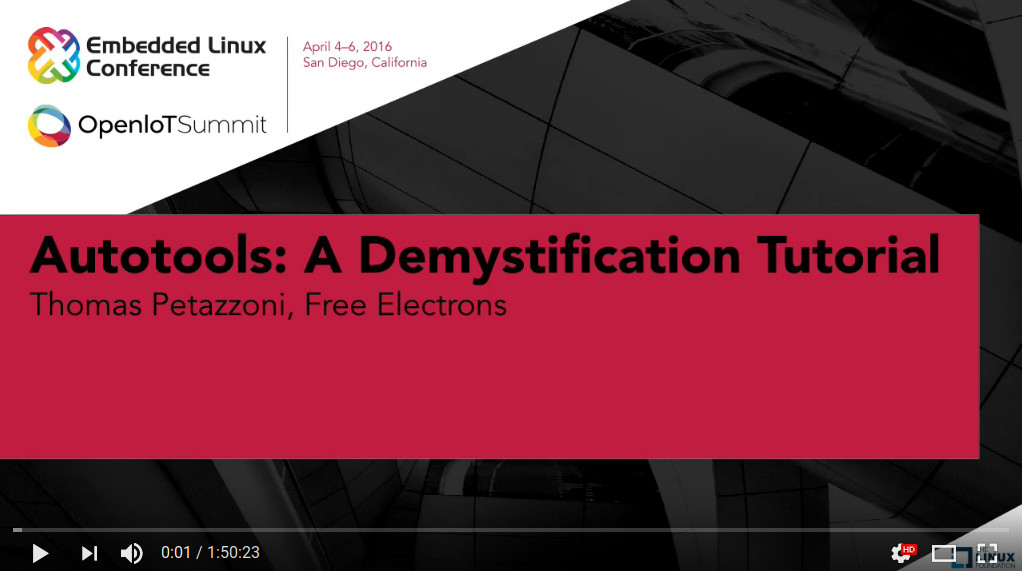
\includegraphics[width=0.5\textwidth]{slides/sysdev-embedded-linux/autotools-tutorial-video-thumbnail.jpg}
\end{frame}

\setuplabframe
{Third party libraries and applications}
{
  \begin{itemize}
  \item Manually cross-compiling applications and libraries
  \item Learning about common techniques and issues.
  \item Compile and run an audio player application!
  \end{itemize}
}

\begin{frame}
  \frametitle{System building tools: principle}
  \begin{itemize}
  \item Different tools are available to automate the process of
    building a target system, including the kernel, and sometimes the
    toolchain.
  \item They automatically download, configure, compile and install
    all the components in the right order, sometimes after applying
    patches to fix cross-compiling issues.
  \item They already contain a large number of packages, that should
    fit your main requirements, and are easily extensible.
  \item The build becomes reproducible, which allows to easily change
    the configuration of some components, upgrade them, fix bugs, etc.
  \end{itemize}
\end{frame}

\begin{frame}
  \frametitle{Available system building tools} Large choice of tools
  \small
  \begin{itemize}
  \item {\bf Buildroot}, developed by the community\\
    \url{http://www.buildroot.org}\\
    See our dedicated course and training materials:
    \url{http://bootlin.com/training/buildroot/}
  \item {\bf PTXdist}, developed by Pengutronix\\
    \url{http://pengutronix.de/en/software/ptxdist.html}
  \item {\bf OpenWRT}, originally a fork of Buildroot for wireless routers,
    now a more generic project\\
    \url{http://www.openwrt.org}
  \item {\bf OpenEmbedded}, more flexible but also far more complicated\\
    \url{http://www.openembedded.org}, its industrialized version {\bf
      Yocto Project} and vendor-specific derivatives such as {\bf Arago}.\\
      See our dedicated course and training materials: 
      \url{http://bootlin.com/training/yocto/}.
  \end{itemize}
\end{frame}

\begin{frame}
  \frametitle{Buildroot (1)}
  \begin{itemize}
  \item Allows to build a toolchain, a root filesystem image with many
    applications and libraries, a bootloader and a kernel image
    \begin{itemize}
    \item Or any combination of the previous items
    \end{itemize}
  \item Supports building uClibc, glibc and musl toolchains,
    either built by Buildroot, or external
  \item Over 2000+ applications or libraries integrated, from basic
    utilities to more elaborate software stacks: X.org, GStreamer, Qt,
    Gtk, WebKit, Python, PHP, etc.
  \item Good for small to medium embedded systems, with a fixed set of
    features
    \begin{itemize}
    \item No support for generating packages (\code{.deb} or
      \code{.ipk})
    \item Needs complete rebuild for most configuration changes.
    \end{itemize}
  \item Active community, releases published every 3 months.
  \end{itemize}
\end{frame}

\begin{frame}
  \frametitle{Buildroot (2)}
  \begin{columns}
    \column{0.6\textwidth}
    \begin{itemize}
    \item Configuration takes place through a \code{*config} interface similar to the
      kernel\\
      \code{make menuconfig}
    \item Allows to define
      \begin{itemize}
      \item Architecture and specific CPU
      \item Toolchain configuration
      \item Set of applications and libraries to integrate
      \item Filesystem images to generate
      \item Kernel and bootloader configuration
      \end{itemize}
    \item Build by just running\\
      \code{make}
    \end{itemize}
    \column{0.4\textwidth}
    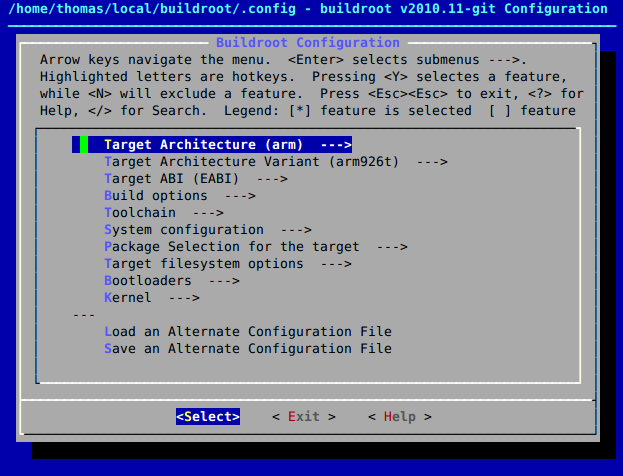
\includegraphics[width=\textwidth]{slides/sysdev-embedded-linux/buildroot-screenshot.png}
  \end{columns}
\end{frame}

\begin{frame}
  \frametitle{Buildroot: adding a new package (1)}
  \begin{itemize}
  \item A package allows to integrate a user application or library to
    Buildroot
  \item Each package has its own directory (such as
    \code{package/gqview}). This directory contains:
    \begin{itemize}
    \item A \code{Config.in} file (mandatory), describing the
      configuration options for the package. At least one is needed to
      enable the package. This file must be sourced from
      \code{package/Config.in}
    \item A \code{gqview.mk} file (mandatory), describing how the
      package is built.
    \item A \code{.hash} file (optional, but recommended), containing
      hashes for the files to download.
    \item Patches (optional). Each file of the form
      \code{*.patch} will be applied as a patch.
    \end{itemize}
  \end{itemize}
\end{frame}

\begin{frame}[fragile]
  \frametitle{Buildroot: adding a new package (2)}
  \begin{itemize}
  \item For a simple package with a single configuration option to
    enable/disable it, the \code{Config.in} file looks like:
\footnotesize
\begin{block}{}
\begin{verbatim}
config BR2_PACKAGE_GQVIEW
        bool "gqview"
        depends on BR2_PACKAGE_LIBGTK2
        help
          GQview is an image viewer for Unix operating systems

          http://prdownloads.sourceforge.net/gqview
\end{verbatim}
\end{block}
\normalsize
  \item It must be sourced from \code{package/Config.in}:
\small
\begin{block}{}
\begin{verbatim}
source "package/gqview/Config.in"
\end{verbatim}
\end{block}
  \end{itemize}
\end{frame}

\begin{frame}[fragile]
  \frametitle{Buildroot: adding new package (3)}
  \begin{itemize}
  \item Create the \code{gqview.mk} file to describe the build steps
\scriptsize
\begin{block}{}
\begin{verbatim}
GQVIEW_VERSION = 2.1.5
GQVIEW_SOURCE = gqview-$(GQVIEW_VERSION).tar.gz
GQVIEW_SITE = http://prdownloads.sourceforge.net/gqview
GQVIEW_DEPENDENCIES = host-pkgconf libgtk2
GQVIEW_CONF_ENV = LIBS="-lm"
GQVIEW_LICENSE = GPL-2.0
GQVIEW_LICENSE_FILES = COPYING

$(eval $(autotools-package))
\end{verbatim}
\end{block}
\normalsize
\item The package directory and the prefix of all variables must be
  identical to the suffix of the main configuration option
  \code{BR2_PACKAGE_GQVIEW}
\item The \code{autotools-package} infrastructure knows how to build
  autotools packages. A more generic \code{generic-package}
  infrastructure is available for packages not using the autotools
  as their build system.
\end{itemize}
\end{frame}

\begin{frame}
  \frametitle{OpenEmbedded / Yocto Project}
  \begin{itemize}
  \item The most versatile and powerful embedded Linux build system
    \begin{itemize}
    \item A collection of recipes (\code{.bb} files)
    \item A tool that processes the recipes: \code{bitbake}
    \end{itemize}
  \item Integrates 2000+ application and libraries, is highly
    configurable, can generate binary packages to make the system
    customizable, supports multiple versions/variants of the same
    package, no need for full rebuild when the configuration is
    changed.
  \item Configuration takes place by editing various configuration
    files
  \item Good for larger embedded Linux systems, or people looking for
    more configurability and extensibility
  \item Drawbacks: very steep learning curve, very long first build.
  \end{itemize}
\end{frame}

\begin{frame}
  \frametitle{Distributions - Debian}
  \small
  \begin{columns}[T]
    \column{0.8\textwidth}
    Debian GNU/Linux, \url{http://www.debian.org}
    \begin{itemize}
    \item Provides the easiest environment for quickly building prototypes
          and developing applications. Countless runtime and
          development packages available.
    \item But probably too costly to maintain
          and unnecessarily big for production systems.
    \item Available on ARM (\code{armel}, \code{armhf}, \code{arm64}),
          MIPS and PowerPC architectures
    \item Software is compiled natively by default.
    \item Use the \code{debootstrap} command to build a root
          filesystem for your architecture, with a custom selection
	  of packages.
    \end{itemize}
    \column{0.2\textwidth}
    %% Debian logo found on
    %https://commons.wikimedia.org/wiki/File:Debian-OpenLogo.svg
    
\includegraphics[width=\textwidth]{slides/sysdev-embedded-linux/Debian-OpenLogo.pdf}\\
  \end{columns}
\end{frame}

\begin{frame}
  \frametitle{Distributions - Others}
  \begin{columns}[T]
    \column{0.7\textwidth}
    Fedora
    \begin{itemize}
    \item \url{http://fedoraproject.org/wiki/Architectures/ARM}
    \item Supported on various recent ARM boards (such as Beaglebone
      Black and Raspberry Pi)
    \item Supports QEMU emulated ARM boards too (Versatile Express board)
    \item Shipping the same version as for desktops!
    \end{itemize}
    \column{0.3\textwidth}
    
\includegraphics[width=\textwidth]{slides/sysdev-embedded-linux/fedora.pdf}\\
    \tiny Image credits: \url{https://bit.ly/2EzmJLF}
  \end{columns}
\end{frame}

\begin{frame}
  \frametitle{Embedded distributions}
  Even if you don't use them for final products, they can be useful
  to make demos quickly
  \small
  \begin{columns}
    \column{0.8\textwidth}
    \begin{itemize}
    \item {\bf Android}: \url{http://www.android.com/}\\
      Google's distribution for phones, tablets, TVs, cars...\\
      Except the Linux kernel, very different user space
      than other Linux distributions. Very successful,
      lots of applications available (many proprietary).
    \item {\bf Alpine Linux}: \url{https://www.alpinelinux.org/}\\
      Security oriented distribution based on {\em Musl}
      and {\em BusyBox}, fitting in about 130 MB of storage,
      supporting x86 and arm, both 32 and 64 bit.
    \end{itemize}
    \column{0.2\textwidth}
    
\includegraphics[width=\textwidth]{slides/sysdev-embedded-linux/android.png}\\
    
\includegraphics[width=\textwidth]{slides/sysdev-embedded-linux/alpinelinux-logo.pdf}\\
  \end{columns}
\end{frame}

\begin{frame}
  \frametitle{Application frameworks}
  \small
  \begin{columns}
    \column{0.8\textwidth}
    Not real distributions you can download. Instead, they
    implement middleware running on top of the Linux kernel
    and allowing to develop applications.
    \begin{itemize}
    \item {\bf Mer}: \url{http://merproject.org/}\\
      Fork from the Meego project.\\
      Targeting mobile devices.\\
      Supports x86, ARM and MIPS. \\
      See \url{http://en.wikipedia.org/wiki/Mer\_(software\_distribution)}
    \item {\bf Tizen}: \url{https://www.tizen.org/} \\
      Targeting smartphones, tablets, netbooks, smart TVs and
      In Vehicle Infotainment devices.\\
      Supported by big phone manufacturers and operators \\
      HTML5 base application framework. \\
      See \url{http://en.wikipedia.org/wiki/Tizen}
    \end{itemize}
    \column{0.2\textwidth}
    
\includegraphics[width=\textwidth]{slides/sysdev-embedded-linux/mer.png}\\
    
\includegraphics[width=\textwidth]{slides/sysdev-embedded-linux/tizen.png}\\
  \end{columns}
\end{frame}

\setuplabframe
{Buildroot}
{
  \begin{itemize}
  \item Rebuild the same system, this time with Buildroot.
  \item See how easier it gets!
  \end{itemize}
}

